\chapter{INTRODUCTION}\label{chap:intro}

\section{Biosecurity and Policies}

The global community faces an escalating array of biological threats that transcend traditional boundaries between nations, economic sectors, and scientific disciplines. The COVID-19 pandemic demonstrated these threats' devastating consequences, causing millions of deaths worldwide and imposing trillions of dollars in economic losses \citep{WHO2021, Hulme2021}. Modern society's interconnected nature—characterized by rapid international travel and extensive trade networks—means biological threats can spread with alarming speed, requiring coordinated responses that integrate public health measures, border controls, surveillance systems, and emergency management protocols \citep{WTO2024}.

The World Health Organization defines biosecurity as a strategic and integrated approach to analyzing and managing relevant risks to human, animal, and plant life and health, along with associated environmental risks \citep{WHO2021}. This comprehensive perspective recognizes connections among human health, animal health, plant health, and ecosystem integrity, often referred to as the One Health approach \citep{Hulme2021}. The Food and Agriculture Organization emphasizes that biosecurity encompasses policy and regulatory frameworks that analyze and manage risks in food safety, animal life and health, and plant life and health \citep{FAO2023}. Effective biosecurity requires coordination across multiple sectors including agriculture, veterinary medicine, public health, environmental protection, customs and border control, transportation, and increasingly, information technology and cybersecurity.

Biosecurity governance operates through a complex architecture of international agreements and national regulations. At the global level, the World Health Organization's International Health Regulations establish binding obligations for member states to develop core capacities for detecting, assessing, reporting, and responding to public health emergencies \citep{WHO2021}. The World Organisation for Animal Health, the Codex Alimentarius Commission, and other international bodies develop standards that member states use as reference points for managing biosecurity risks \citep{WTO2024}. The Biological Weapons Convention prohibits the development, production, and stockpiling of biological weapons, establishing a standard-setting foundation against the harmful use of biological agents \citep{UNODA2023}.

Malaysia has implemented comprehensive biosecurity policies reflecting both its exposure to biological threats and its strategic position in global trade networks. As a tropical country with extensive agricultural production and a major exporter of agricultural commodities including palm oil and rubber, Malaysia faces biosecurity risks from endemic diseases, imported pests and pathogens, and potential bioterrorism \citep{Malaysia2023}. The country's location along the Strait of Malacca—through which approximately one-quarter of global maritime trade transits—positions it as a critical node in international supply chains and a potential entry point for biological threats \citep{ASEAN2024}.

Recognizing cybersecurity's growing importance to national security and economic competitiveness, Malaysia enacted the Cybersecurity Act 2024, which came into force on 26 August 2024 \citep{Malaysia2024}. This landmark legislation establishes a comprehensive framework for managing cybersecurity risks to critical information infrastructure, including systems supporting biosecurity functions. The Act designates the National Cyber Security Agency as the lead authority for coordinating cybersecurity policy and incident response, with powers to designate systems as National Critical Information Infrastructure and to require their operators to implement cybersecurity measures, report incidents, and undergo regular audits \citep{NACSA2024}. The legislation applies beyond national borders to cybersecurity service providers whose activities affect Malaysia's cybersecurity, reflecting the cross-border nature of cyber threats \citep{CMS2024}.

Malaysia has also established regulatory frameworks for unmanned aerial systems. The Civil Aviation Authority of Malaysia enforces comprehensive drone regulations under the Malaysian Civil Aviation Regulations 2016, which categorize unmanned aircraft based on weight and operational characteristics \citep{CAAM2024}. Small Unmanned Aircraft Systems weighing up to 20 kilograms are subject to relatively flexible regulations for recreational use, while commercial operations require permits with specific requirements for operator qualifications, aircraft certification, and insurance coverage \citep{DroneAcademy2023}. Several locations have been designated as no-fly zones for security purposes, including Putrajaya, the Kuala Lumpur City Centre, Parliament House, and military installations \citep{DroneRegulations2024}.

Biosecurity encompasses multiple linked types addressing different categories of biological threats. Agricultural biosecurity protects crops, livestock, and aquaculture from pests and diseases through quarantine inspections, certification programs, pest surveillance systems, and rapid response protocols \citep{FAO2023}. Public health biosecurity addresses infectious disease threats to human populations through disease surveillance systems, laboratory networks, stockpiles of medical countermeasures, and health system surge capacity \citep{WHO2021}. Environmental biosecurity protects ecosystems and biodiversity from invasive alien species and genetically modified organisms \citep{Hulme2021}. Laboratory biosecurity ensures secure storage and handling of dangerous pathogens through biosafety regulations and inventory management systems.

Figure \ref{fig:biosecurity_types} illustrates the major types of biosecurity and their relationships, with particular emphasis on cybersecurity's central role in enabling and protecting biosecurity functions across all domains.

\begin{figure}[htbp]
	\centering
	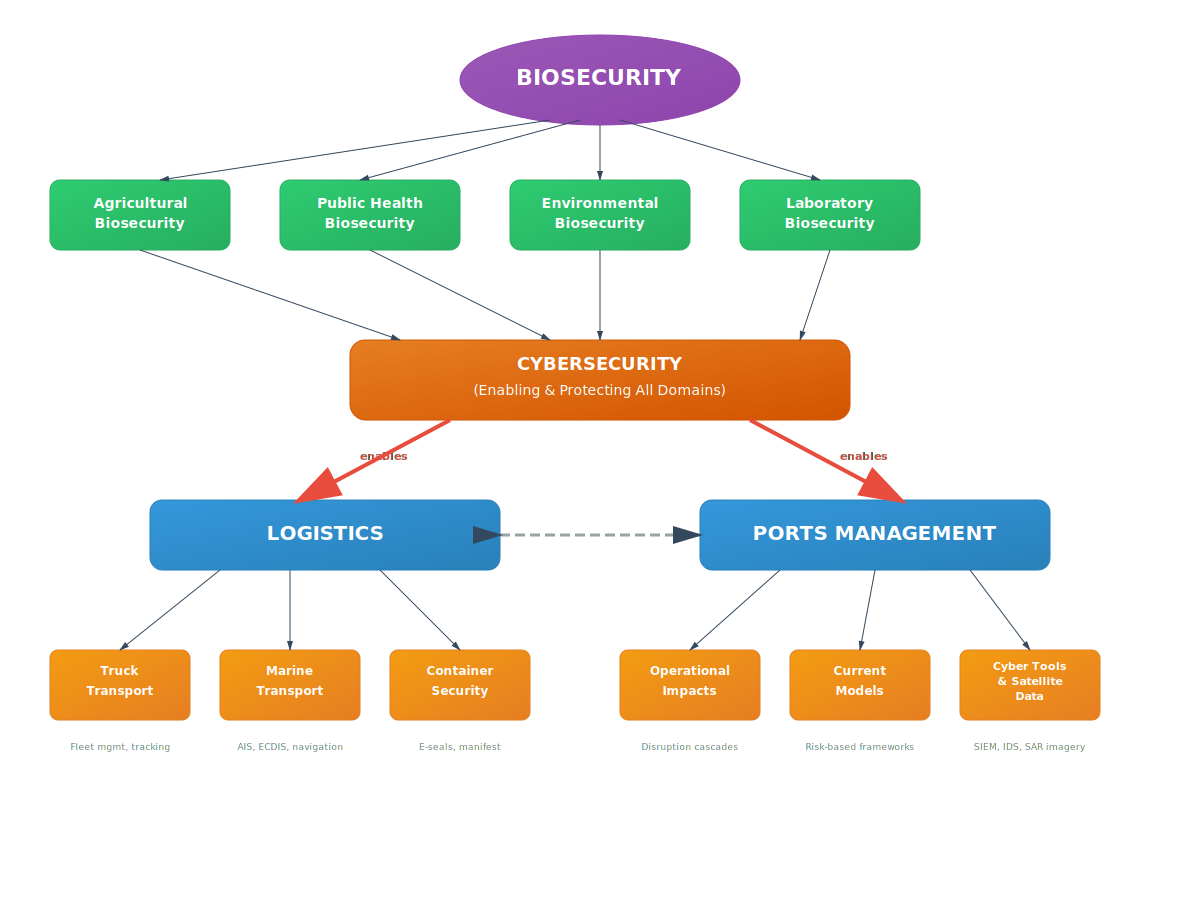
\includegraphics[width=0.90\textwidth]{figures/biosecurity_types_framework.png}
	\caption{Types of Biosecurity and the Central Role of Cybersecurity}
	\label{fig:biosecurity_types}
\end{figure}

Within the broader biosecurity landscape, cybersecurity has emerged as a critical enabling capability underpinning biosecurity measures' effectiveness across all domains. Modern biosecurity systems increasingly depend on digital technologies for surveillance, data management, communication, laboratory analysis, and coordination of response activities \citep{ENISA2023}. Disease surveillance systems collect and analyze vast quantities of data from healthcare facilities and laboratories to detect outbreaks early and track their spread. Border control systems use databases, risk assessment algorithms, and electronic cargo tracking to target inspections at high-risk shipments while facilitating legitimate trade. Laboratory information management systems maintain inventories of dangerous pathogens and track specimen transfers. Emergency management systems coordinate personnel and resource deployment during outbreaks. These digital systems create dependencies on cybersecurity—their compromise could blind surveillance systems to emerging threats, misdirect response resources, or enable theft of dangerous pathogens.

Cybersecurity intersects with biosecurity through two critical domains essential to global commerce and public health: logistics operations and ports management. Modern logistics systems rely on information technologies to coordinate goods movement across supply chains spanning multiple countries and transportation modes \citep{Notteboom2024}. Truck transportation increasingly employs digital fleet management systems, electronic logging devices, and real-time cargo tracking technologies that enhance operational efficiency but create cybersecurity vulnerabilities \citep{DHS2024}. Marine transportation has adopted automatic identification systems, electronic chart display and information systems, and satellite communications that improve safety and efficiency but also create attack surfaces for cyber intrusions \citep{IMO2022}. Container shipping relies heavily on digital systems including electronic cargo manifests, automated risk assessment algorithms, electronic seals, and tracking systems throughout the supply chain \citep{WCO2023}.

Ports management represents a particularly critical nexus of cybersecurity and biosecurity concerns given ports' role as gateways for international trade and potential entry points for biological threats. Modern ports function as complex cyber-physical systems integrating information technology, operational technology, and physical infrastructure \citep{Notteboom2024}. Terminal operating systems coordinate container movements, port community systems facilitate information sharing among multiple organizations, vessel traffic management systems monitor ship movements, and cargo screening technologies enable non-intrusive inspection for contraband including dangerous biological materials. The 2017 NotPetya ransomware attack on Maersk Line demonstrated global shipping infrastructure's vulnerability, costing approximately 300 million US dollars and forcing shutdown of 76 container terminals \citep{Lloyd2018}. The 2023 ransomware attack on the Port of Nagoya forced suspension of container operations for four days \citep{MarineDigital2023}.

Current operational models for port management increasingly recognize cybersecurity as a fundamental component of port security. Leading port authorities have adopted risk-based cybersecurity frameworks aligned with international standards including the International Maritime Organization's Guidelines on Maritime Cyber Risk Management, the National Institute of Standards and Technology Cybersecurity Framework, and ISO/IEC 27001 \citep{IMO2022, NIST2023, ISO27001}. Tools and technologies for port cybersecurity include network security solutions such as firewalls and intrusion detection systems, industrial control system security technologies for operational technology environments, security information and event management platforms, endpoint detection and response solutions, and vulnerability assessment tools \citep{ENISA2023}.

Terrain and satellite data play increasingly important roles in port security by providing capabilities for monitoring port facilities and tracking vessel movements. Satellite-based automatic identification systems enable global tracking of ship movements for maritime domain awareness and security surveillance \citep{IMO2022}. Synthetic aperture radar satellites provide all-weather imagery of port facilities and surrounding waters, while optical satellite imagery enables detailed monitoring of port infrastructure and vessel identification \citep{ESA2023}. However, reliance on space-based systems creates potential vulnerabilities if satellite systems are disrupted by technical failures or deliberate attacks \citep{DHS2024}.

This thesis addresses the critical need for efficient, reliable, and secure pathfinding capabilities for autonomous vehicles operating in biosecurity-sensitive environments such as agricultural facilities, healthcare settings, transportation hubs, and border control operations. The research develops novel algorithms for grid-based pathfinding that reduce computational complexity while maintaining path quality and enabling real-time responsiveness to dynamic environment changes. Particular attention is devoted to risk-aware pathfinding that minimizes exposure to contaminated or high-risk areas, a capability essential for autonomous systems operating in biosecurity contexts where human safety and mission effectiveness depend on avoiding known or suspected biosecurity hazards.


\section{Problem Statement}

Deploying autonomous systems for grid-based navigation faces several interconnected challenges that limit their effectiveness and practical utility, particularly in time-critical and risk-sensitive applications. This section identifies four key problems that significantly constrain current autonomous navigation capabilities.

\textbf{Problem 1: Real-time Computational Constraints.} Standard pathfinding algorithms face a fundamental challenge when applied to large-scale or highly cluttered environments: computation time grows prohibitively as problem complexity increases. On large grids, the state space expands quadratically with environment dimensions, forcing algorithms to examine vast numbers of potential paths before finding acceptable solutions. This computational burden becomes particularly severe in risk-annotated grids commonly used for biosecurity applications, where each cell contains not only traversability information but also exposure data requiring evaluation of composite cost functions that balance distance against risk metrics. The problem intensifies in cluttered environments featuring narrow aisles or complex obstacle configurations, where algorithms must explore numerous alternative routes before identifying feasible paths. In time-critical missions such as biosecurity surveillance, rapid response to detected contamination, or emergency disinfection operations, these computational delays directly impact mission effectiveness. When autonomous systems cannot compute paths quickly enough to respond to evolving situations, the resulting hesitation or inability to react can compromise operational objectives and potentially endanger human operators or critical assets that depend on timely autonomous system deployment.

\textbf{Problem 2: Limited Adaptability to Dynamic Environments.} Real-world operational environments rarely remain static. Occupancy and risk information frequently change due to moving obstacles, personnel activity, updated sensor readings, new test results, and evolving contamination zones. In biosecurity contexts specifically, risk maps may require updates based on newly detected pathogens, revised quarantine boundaries, or temporal progression of contamination spread. Current planning approaches struggle with this inherent dynamism. When environmental conditions change, most systems must restart the entire planning process from the beginning, discarding all previously computed information. This complete restart incurs substantial computational overhead, especially problematic when updates occur frequently or when environments are large and complex. The delays introduced by repeated full re-planning become critical bottlenecks in time-sensitive scenarios where rapid adaptation maintains safety margins and mission effectiveness. Beyond the computational costs, frequent complete re-planning can produce inconsistent or oscillating path selections as the system responds to each new environmental state, potentially confusing human operators who must supervise autonomous operations or compromising autonomous system reliability when paths change dramatically in response to minor environmental updates. The fundamental issue is that current systems lack mechanisms to efficiently update existing plans by incorporating only locally relevant changes, instead treating every environmental modification—however small—as requiring complete plan reconstruction.

\textbf{Problem 3: Significant Deployment and Integration Barriers.} Despite extensive research on grid-based pathfinding algorithms and their thorough evaluation in simulation environments, a substantial gap exists between algorithmic development and practical deployment on physical autonomous vehicles. This gap manifests in multiple dimensions that collectively impede technology transfer from research to operational systems. First, there is limited availability of accessible, well-documented toolchains that integrate grid-based planning algorithms with actual vehicle control systems, particularly for scenarios requiring risk-aware navigation. Researchers and practitioners face significant barriers when attempting to bridge from abstract algorithmic implementations to systems that can command real vehicles. Second, converting abstract grid paths into executable vehicle trajectories requires careful attention to vehicle dynamics, control system constraints, and safety margins—aspects often neglected in purely algorithmic research focused on optimality metrics like path length or computation time. The practical reality of autonomous vehicle control introduces complexities that simulation environments may not capture adequately. Third, validating and testing integrated planning-execution systems typically demands access to specialized hardware, facilities, and expertise not readily available to many researchers or practitioners interested in deploying advanced pathfinding techniques. In biosecurity robotics particularly, where safe and reproducible execution is paramount for tasks such as contamination surveillance transects, targeted sampling route navigation, and systematic disinfection operations, this deployment barrier represents a critical obstacle. The absence of validated, accessible pipelines demonstrating reliable path execution even in realistic simulation environments impedes the transition from research prototypes to operational systems that biosecurity personnel could actually deploy in field conditions.

\textbf{Problem 4: Unexploited Structural Regularities in Operational Environments.} Many practical autonomous navigation scenarios occur in structured facilities that exhibit inherent geometric regularities, particularly horizontal symmetries in environments such as greenhouses, warehouses, hospital wards, agricultural storage facilities, and similar structured spaces. These environments typically feature parallel rows, corridors, or aisles creating symmetric patterns in their spatial organization. Classical pathfinding algorithms, however, treat each location as an independent state without recognizing or exploiting these structural regularities. This limitation results in substantial redundant computation, as algorithms independently explore symmetric regions that could potentially be processed collectively. The computational inefficiency becomes particularly pronounced in large-scale structured environments where symmetry is prevalent and predictable. Moreover, in risk-annotated grids where symmetry extends beyond geometric layout to include similar risk distributions in symmetric regions, the failure to exploit symmetry represents a missed opportunity not only for computational efficiency but also for ensuring consistent risk-cost evaluation across structurally equivalent portions of the environment. Current systems perform extensive redundant calculations exploring symmetric regions as if they were unrelated, consuming computational resources that could be allocated to more complex aspects of path planning or to enable faster response times. This fundamental inefficiency particularly constrains applications requiring real-time performance in structured environments where symmetry could provide substantial computational advantages if properly recognized and exploited.


\section{Research Questions and Research Hypotheses}

Based on the problems identified in Section 1.2, this research formulates four research questions and corresponding hypotheses that guide the development, implementation, and evaluation of the proposed pathfinding techniques.

\textbf{Research Question 1 (RQ1):} To what extent can constraining search to an Incremental Line Search (ILS) corridor reduce computational requirements and cumulative exposure while preserving path optimality on risk-annotated grid maps?

\textbf{Research Hypothesis 1 (RH1):} The ILS approach will achieve significant reductions in runtime and node expansions (expected reduction of 40-70\% compared to standard A*) while maintaining path lengths within 5\% of optimal solutions. Additionally, on risk-annotated grids, ILS will reduce the cumulative exposure integral (sum of risk values along the path) by prioritizing paths through the corridor that naturally avoid high-risk regions, with negligible impact on path quality as measured by standard optimality metrics.

\textbf{Research Question 2 (RQ2):} Can an adaptive corridor mechanism that dynamically adjusts ILS corridor width based on local obstructions and risk concentrations support efficient re-planning under dynamic environmental updates while maintaining exposure constraints?

\textbf{Research Hypothesis 2 (RH2):} An adaptive corridor widening strategy that expands the search space only near detected obstructions or risk spikes will sustain the computational advantages of ILS (maintaining 50-80\% of the speedup observed in static scenarios) while successfully handling moderate environment dynamics. The adaptive mechanism will keep cumulative exposure within user-specified thresholds (e.g., no more than 15\% increase in exposure integral) even under dynamic updates, and will achieve re-planning latencies that are 3-5 times faster than complete re-planning approaches.

\textbf{Research Question 3 (RQ3):} Does an open-source planning-to-flight pipeline integrating ILS with risk-aware cost functions and ArduPilot Software-In-The-Loop (SITL) simulation reliably execute grid-derived paths for autonomous vehicles?

\textbf{Research Hypothesis 3 (RH3):} The integrated planning-to-flight pipeline will successfully execute planned paths in ArduPilot SITL with bounded tracking errors (position error $<$ 2 meters for waypoint following) and successful task completion rates exceeding 95\% for typical biosecurity mission profiles including surveillance transects, sampling routes, and disinfection patterns. The pipeline will demonstrate reproducible execution across multiple simulation runs with consistent performance metrics, providing a validated foundation for safe hardware deployment when permitted by safety protocols and regulatory requirements.

\textbf{Research Question 4 (RQ4):} When horizontal symmetry exists in grid environments, does the Folding A* algorithm provide predictable constant-factor acceleration while preserving optimality and correctly handling risk-weighted costs?

\textbf{Research Hypothesis 4 (RH4):} On horizontally symmetric grids, Folding A* will achieve approximately 50\% reduction in the effective state space (i.e., exploring roughly half the nodes compared to standard A*) with exact optimality preservation for both standard and risk-weighted cost functions. The runtime improvements will scale consistently across different grid sizes and obstacle densities, yielding speedups ranging from 1.8x to 2.2x compared to standard A* on symmetric maps. The algorithm will correctly handle risk-annotated grids by maintaining symmetry-aware risk propagation, ensuring that paths in symmetric regions are evaluated with equivalent composite costs.


\section{Research Objectives}

The overarching aim of this research is to develop, implement, and validate efficient grid-based pathfinding techniques for autonomous systems that combine computational efficiency with practical deployability, particularly in risk-sensitive biosecurity applications. This aim is achieved through four specific research objectives:

\textbf{Objective 1 (O1):} Design and evaluate an Incremental Line Search (ILS) framework for risk-aware pathfinding that focuses exploration within a narrow corridor centered on a direct line between start and goal positions. The framework must integrate seamlessly with standard grid planning algorithms (A*, Dijkstra, BFS), support optional risk-weighted cost functions, and demonstrate measurable reductions in runtime and node expansions while maintaining near-optimal path quality. The evaluation will encompass diverse grid scenarios including varying sizes (50x50 to 1000x1000), obstacle densities (10\%-40\%), and risk annotation patterns reflecting realistic biosecurity scenarios such as quarantine zones and contamination gradients.

\textbf{Objective 2 (O2):} Develop and validate an adaptive corridor control mechanism for ILS that dynamically adjusts corridor width based on local environmental features including obstacle concentrations and risk-level spikes. The adaptive mechanism must balance exploration efficiency with solution completeness, ensuring that narrow corridors are used in open regions while sufficient expansion occurs near obstructions or high-risk zones. The control strategy will be evaluated under dynamic environments with piecewise-static updates at various frequencies (1-10 updates per planning session), assessing its ability to maintain computational efficiency while preserving path quality and exposure constraints across update cycles.

\textbf{Objective 3 (O3):} Implement and formally validate the Folding A* algorithm for horizontally symmetric grid maps, providing rigorous proofs of correctness and optimality preservation for both standard and risk-weighted cost functions. The implementation must include automatic symmetry detection mechanisms, efficient folding transformations that halve the effective state space, and correct unfolding procedures to recover full-space paths. The empirical evaluation will quantify constant-factor speedup gains across diverse symmetric grid scenarios, analyzing how performance scales with grid size, obstacle density, and the degree of symmetry in the environment.

\textbf{Objective 4 (O4):} Build and release an open-source, end-to-end grid-planning-to-flight pipeline that integrates ILS and Folding A* algorithms with ArduPilot Software-In-The-Loop (SITL) simulation for autonomous vehicle execution. The pipeline must support risk-annotated grid inputs, automatic conversion of grid paths to vehicle waypoints with appropriate safety margins, and comprehensive logging for performance analysis. The implementation will be validated through systematic SITL experiments demonstrating successful execution of representative biosecurity mission profiles including surveillance transects, area coverage patterns, and targeted sampling or disinfection routes. The pipeline will be released under a permissive open-source license to facilitate community adoption and extension.


\section{Scope and Limitations}

This research focuses on grid-based pathfinding for autonomous navigation with specific scope boundaries and acknowledged limitations defining the results' applicability and generalizability.

\textbf{Environment Representation:} The research considers two-dimensional occupancy grids with optional risk layers. Grid cells are classified as either traversable or occupied, with traversable cells optionally annotated with continuous risk values normalized to [0, 1]. The evaluation encompasses grid sizes from 50x50 to 1000x1000 cells and obstacle densities from 10\% to 40\%. Risk distributions include uniform random patterns, localized hotspots, and structured zones reflecting quarantine areas or contamination gradients. Full three-dimensional environments with varying altitude constraints are considered out of scope.

\textbf{Agent Model:} The research assumes a single autonomous agent with either 4-connected or 8-connected motion primitives. For aerial vehicles, a fixed-altitude abstraction is employed. The agent is modeled as occupying a single grid cell at any discrete time step. Vehicle dynamics and continuous-time trajectory optimization are addressed at the execution layer rather than in the planning phase. Multi-agent coordination is explicitly excluded.

\textbf{Environment Dynamics:} The research considers moderate, piecewise-static dynamics where occupancy and risk updates occur at discrete time points with sufficient intervals for the planner to complete computation. The evaluation includes scenarios with 1 to 10 updates per planning session. Highly adversarial dynamics and continuous-time stochastic environment evolution are out of scope.

\textbf{Planning Objectives:} The primary objective is to find collision-free paths from start to goal subject to real-time latency constraints. For standard grids, path cost is cumulative distance based on Euclidean or Manhattan metrics. For risk-annotated grids, a composite cost function combines distance with weighted risk: $cost = distance + \lambda \cdot \sum risk$, where $\lambda$ is a user-specified weight parameter. The research evaluates multiple $\lambda$ values to assess sensitivity to risk-cost tradeoff preferences.

\textbf{Evaluation Metrics:} Performance assessment employs runtime (wall-clock computation time), nodes expanded, path length, exposure integral (sum of risk values along the path), maximum on-path risk, and re-plan latency. All experiments are conducted on controlled hardware configurations (Intel Core i7 or equivalent, 16GB RAM) to ensure reproducibility.

\textbf{Input Assumptions:} The research assumes that occupancy information and optional risk annotations are provided as external inputs from perception systems. The source of this information, sensor fusion techniques, and uncertainty quantification are not addressed. Start and goal positions are assumed known and specified in advance.

\textbf{Limitations:} The computational gains of corridor-constrained ILS may diminish on highly winding or twisted maps. Folding A* provides benefits only when horizontal symmetry is present and detectable. Risk-map uncertainty modeling is not explicitly addressed. The ArduPilot SITL integration provides validation in simulation but does not replace the need for comprehensive hardware testing before operational deployment.


\section{Significance of the Research}

This research makes significant contributions to both theoretical understanding and practical deployment of autonomous navigation systems, with particular relevance to biosecurity applications.

\textbf{Computational Efficiency:} The proposed corridor-constrained ILS approach dramatically reduces the search space requiring exploration to find high-quality paths. By constraining exploration to a narrow corridor around the direct line between start and goal, ILS enables real-time pathfinding on large-scale grids using commodity hardware, without requiring specialized processors or GPU acceleration. For time-critical applications such as emergency response or surveillance of sudden contamination events, computing paths within strict latency constraints can significantly enhance operational capability.

\textbf{Enhanced Safety:} Integrating risk-annotated grids with ILS and Folding A* enables autonomous systems to balance competing objectives of efficiency and safety in contaminated or hazardous environments. Explicitly treating exposure integrals and maximum on-path risk provides quantifiable safety metrics that can be incorporated into mission planning. By reducing average exposure while maintaining acceptable path lengths, the proposed techniques enable more aggressive deployment of autonomous systems in scenarios where human access would pose unacceptable safety risks.

\textbf{Improved Responsiveness:} The adaptive corridor mechanism specifically addresses efficient re-planning challenges under dynamic environment changes. By enabling localized corridor widening only where necessary, the adaptive approach maintains ILS computational efficiency while ensuring solution completeness under moderate dynamics. This capability is particularly valuable in biosecurity operations where risk maps are frequently updated based on new test results or revised contamination boundaries.

\textbf{Predictable Performance:} Folding A* makes a fundamental theoretical contribution by demonstrating how horizontal symmetry can be exploited to achieve guaranteed constant-factor state-space reductions while preserving optimality. Unlike heuristic acceleration techniques that may provide variable speedups, the symmetry-based reduction is predictable and analyzable, making it suitable for systems with hard real-time constraints or safety-critical requirements.

\textbf{Practical Deployment Infrastructure:} The open-source planning-to-flight pipeline addresses a critical gap between algorithmic research and practical deployment. Integration with ArduPilot SITL enables researchers and practitioners to evaluate and refine pathfinding algorithms in a realistic simulation environment. This infrastructure reduces barriers to deploying advanced pathfinding techniques on physical vehicles, potentially accelerating technology transfer from research prototypes to operational systems.

\textbf{Broader Impact:} While biosecurity applications provide the primary motivation, the techniques developed in this thesis have broader applicability to general autonomous navigation problems wherever grid-based planning is employed. The ILS corridor-constrained approach can benefit warehouse automation, agricultural robots navigating crop rows, search and rescue operations, and any scenario where rapid pathfinding on large grids is required. Open-source release of implementations and the planning-to-flight pipeline facilitates adoption across diverse application domains.


\section{Organization of the Thesis}

This thesis is organized into seven chapters that systematically develop, implement, and evaluate the proposed pathfinding techniques.

\textbf{Chapter 1: Introduction} provides foundational context including biosecurity challenges and their relationship to autonomous navigation, identification of key problems limiting current approaches, formulation of research questions and hypotheses, specification of research objectives, and definition of scope and limitations.

\textbf{Chapter 2: Literature Review} surveys existing knowledge on classical search algorithms (Dijkstra, BFS, A*), heuristic search techniques, incremental and anytime planning approaches, line-of-sight path shortcutting methods, symmetry exploitation techniques, and risk-sensitive routing methods. The review identifies gaps in current approaches motivating ILS and Folding A* development.

\textbf{Chapter 3: Incremental Line Search Framework} presents detailed design, implementation, and analysis of the ILS corridor-constrained pathfinding approach, including corridor construction algorithms, adaptive widening strategies, integration mechanisms with standard grid planners, theoretical complexity analysis, and benchmark results on risk-aware grid scenarios.

\textbf{Chapter 4: Folding A* for Symmetric Grids} develops the symmetry-aware planning technique, including formal definitions of horizontal symmetry, folding transformation descriptions, comprehensive correctness and optimality proofs, theoretical complexity analysis, and experimental results quantifying speedups across diverse symmetric grids.

\textbf{Chapter 5: Open-Source Planning-to-Flight Pipeline} documents the integrated system bridging grid-based planning with vehicle execution using ArduPilot SITL, including pipeline architecture, path-to-waypoint conversion, ArduPilot interface configuration, and experimental validation demonstrating successful execution of biosecurity mission profiles.

\textbf{Chapter 6: Results and Discussion} provides comprehensive comparative evaluations including comparative performance analysis of ILS versus standard algorithms, evaluation of Folding A* speedups, ablation studies isolating parameter impacts, sensitivity analyses, and practical implications for biosecurity operations.

\textbf{Chapter 7: Conclusions} synthesizes key findings including algorithmic innovations, theoretical results, and empirical findings, discusses limitations including assumptions and cases where proposed techniques may not provide advantages, and identifies promising avenues for future research including extensions to three-dimensional environments, integration with learning-based approaches, and field deployment on physical hardware.